\documentclass[11pt,a4paper]{article}

% --- Packages ---
\usepackage[utf8]{inputenc}
\usepackage[margin=1in]{geometry}
\usepackage{titlesec}
\usepackage{hyperref}
\usepackage{cite}
\usepackage{graphicx}
\usepackage{booktabs} % For professional tables
\usepackage{listings} % For code snippets if needed
\usepackage{tabularx}
\usepackage{url}
\usepackage{float}

% --- Document Info ---
\title{Project Report: Bulk Document Processing and Q\&A using Retrieval-Augmented Generation and Multi-Agent Workflows}
\author{Joseph Moore \\ \small Candidate Number: 2412423}
\date{March 27, 2026}

\begin{document}

\maketitle

\begin{abstract}

The initial problem selected for this project was one of assisting the staff in Small Legal Clinics across the country. These clinics are often massively understaffed and underfunded, leading to people who don't have the financial means to seek a for-profit solicitor to be left stranded, waiting for months, or years, for availability in a free legal clinic. This project's aim is to alleviate some of the work required by the, often voluntary, staff at these clinics, causing wait times to decrease, and giving more people access to the help that they need. This was achieved by building a system that allows some of the less mentally demanding, yet time-intensive activities to be completed more easily, or automatically in certain cases.\par

Following a User-Centred Design Approach, a legal volunteer was interviewed, and a literature review of existing papers related to this problem was conducted. This research highlighted a massive range of factors that must be accounted for, ranging from the need for a low-cost solution to this problem to automatic document drafting and deep research, both of which would otherwise have to be done manually and slowly.

\end{abstract}

\section{Introduction}
\label{sec:intro}

% This covers "Background and motivation"
\subsection{Problem Statement:}

\begin{quote}
"Small Legal Clinics across the country face a systemic crisis: a growing disparity between the high volume of low-income individuals requiring legal counsel and the severely limited human and financial resources available to assist them. Currently, understaffed and often voluntary teams are overwhelmed by administrative overhead and repetitive manual tasks, such as document drafting and preliminary case research. This bottleneck results in excessive wait times - often spanning months or years - effectively denying justice to those who cannot afford it. There is an urgent need for a low-cost technical solution that can automate routine legal workflows without compromising the specific regulatory and data-handling requirements inherent to the legal profession."
\end{quote}

\subsection{Motivation:}

The United Kingdom's legal aid system is currently facing a "pro-bono crisis". While for-profit solicitors have access to expensive, high-end suites of technology, small-scale and voluntary legal clinics remain tethered by manual, paper-heavy workflows. These clinics are the last line of defence for low-income individuals, yet they are consistently underfunded and understaffed. \par

The cost of this disparity is a "justice desert", where vulnerable individuals wait months or years for initial consultations. Through the research and interviews conducted for this project, it became clear that staff are often burdened with administrative tasks, which could be automated. \par

The motivation for this project is to democratize access to high-end legal tools, by providing a solution that returns time to the experts, allowing them to focus on advocacy rather than administration.

\subsection{Aims and Objectives:}

\subsubsection{Aims:}
The primary aim of this project is to design, implement, and evaluate a cost-effective digital assistant tailored to some of the specific workflows of small legal clinics. The focus of this project is on improving the speed of the "intake to draft" pipeline, transforming raw client interviews into structured, legal artifacts, while maintaining strict data privacy standards.

\subsubsection{Objectives:}
To achieve this aim, the following technical and research objectives were established:
\begin{itemize}
    \item \textbf{Requirements Synthesis:} Conduct a semi-structured interview with a volunteer to identify the most time-consuming bottlenecks.
    \item \textbf{Privacy-First Architecture:} Design a system that handles sensitive client data appropriately, to ensure compliance with legal professional privilege.
    \item \textbf{Core Feature Implementation:} \begin{itemize}
        \item \textbf{Automated Summarisation:} Develop a module to extract key legal facts from documents, either structured and official, or from a more unstructured style.
        \item \textbf{Template Driven Drafting:} Create an engine capable of generating formatted legal documents, based on the extracted facts.
    \end{itemize}
    \item \textbf{Performance Evaluation:} Conduct a comparative time-motion study to measure the efficiency gains of the tool, versus traditional manual drafting.
\end{itemize}


\section{Context and Related Work}
\label{sec:context}

\subsection{The Socio-Technical Landscape}

The 2012 LASPO Act severely reduced civil legal aid in England and Wales, shifting the burden of unmet legal needs onto overstretched, volunteer-led pro-bono clinics \cite{laa2023}. This specific environment requires technological interventions to be deployable at near-zero marginal cost, while strictly maintaining client data privacy and producing rigorous, professionally formatted outputs.

\subsection{Academic Literature: NLP in the Legal Domain}

While early automated legal reasoning relied on brittle rule-based systems \cite{mccarty1977}, modern transformer architectures (such as BERT and GPT) have revolutionized the field \cite{vaswani2017, devlin2019, brown2020}, including highly capable models adapted specifically for legal domain tasks \cite{chalkidis2020, bommarito2022}.\par
However, autoregressive models are prone to hallucination---generating plausible but factually unsupported content \cite{maynez2020, ji2023}. In a legal context, this could mislead clients or expose practitioners to regulatory sanctions. To mitigate this, the proposed system utilizes Retrieval-Augmented Generation (RAG) \cite{lewis2020}. This anchors the generative model's outputs in dynamically retrieved, non-parametric knowledge from the user's specific documents, addressing common failure modes of long-context language models \cite{liu2023}.\par
To handle complex legal queries (like drafting letters versus answering questions), the system moves beyond single-chain RAG and employs a Multi-Agent architecture \cite{wu2023}. By dividing the workload into specialised Planner, Retriever, and Responder/Drafter agents, the system isolates reasoning tasks and reduces semantic errors.

\subsection{Competitive Analysis: Commercial vs. General Solutions}

A number of commercial products have emerged in the legal AI market in recent years. Harvey,
a GPT-4-class system trained on legal data and targeted at large law firms, has seen rapid
uptake in BigLaw. Casetext's
CoCounsel (since acquired by Thomson Reuters) and Lexis+~AI (LexisNexis) similarly offer
retrieval-augmented legal research capabilities at a premium price point.
These tools offer output quality attributable to both model scale and legal fine-tuning, but
share a structural characteristic that renders them inaccessible to the target user base of
this project: they are priced for commercial law firm revenue structures and perform inference
on third-party cloud infrastructure, making them unsuitable for handling the sensitive personal
data of legal aid clients under the UK GDPR's data-minimisation and purpose-limitation
obligations~\cite{ico2023}.

General-purpose assistants such as ChatGPT~(OpenAI) and Gemini~(Google) are broadly accessible
and low or zero cost, but carry significant structural limitations for professional legal use:
outputs are not grounded in user-specific documents, inline citation is absent by default (and
unreliable when attempted), and unless enterprise data-processing agreements are in place,
user queries may be used for model training or otherwise processed on external servers.

\begin{table}[h]
\centering
\resizebox{\textwidth}{!}{%
\begin{tabular}{@{}llll@{}}
\toprule
\textbf{Feature} & \textbf{Commercial (e.g., Harvey)} & \textbf{General (e.g., ChatGPT)} & \textbf{Proposed System} \\ \midrule
Cost             & Prohibitive (\$100s/mo)            & Low / Free                       & \textbf{Near-Zero}       \\
Data Privacy     & Enterprise-Grade (cloud)           & Variable / Risky                 & \textbf{Fully Local}     \\
Document Grounding & User files (cloud-stored)        & None (parametric knowledge)      & \textbf{Local RAG}       \\
Output Accuracy  & High (legal fine-tuned)            & Moderate (hallucinations)        & \textbf{Citation-Enforced} \\
Reasoning Transparency & Opaque / proprietary       & None                             & \textbf{Full agent trace} \\ \bottomrule
\end{tabular}%
}
\caption{Comparison of current legal assistance technologies.}
\label{tab:comparison}
\end{table}

\noindent It is acknowledged that the proposed system's generative backbone---gemma3:4b, a 4-billion parameter open-weights model served locally via Ollama---cannot match the absolute output quality of GPT-4-class systems with legal fine-tuning. The system's
competitive proposition is therefore not raw output quality but the combination of local
deployment (all document content and inference remain on the practitioner's machine), near-zero operational cost,
transparent and inspectable agent reasoning, and enforced citation that together are
appropriate for the resource and compliance profile of pro-bono clinical settings.
The one exception to local-only operation is the optional web-search fallback: when no
sufficiently relevant document chunk is found, the user's query string is forwarded to
DuckDuckGo to retrieve supplementary context.  No document content is transmitted;
however, practitioners should be aware that the query text itself leaves the local
environment in this case, and the fallback is surfaced clearly in the frontend alongside
the generated answer.

\subsection{Gap Analysis: The Need for Bespoke Pro-Bono Tech}

The literature review and competitive analysis converge on a single structural tension, here
termed the \textbf{Efficiency--Cost Paradox}: tools with sufficient capability and accuracy
for professional legal work are priced for commercial law firm revenues and process data on
third-party infrastructure incompatible with client confidentiality obligations; conversely,
tools that are free and privacy-preserving lack the document grounding, citation rigour, and
structured output formatting required for their outputs to be used in professional legal
practice without substantial post-generation review.

This paradox is structural rather than a temporary market gap. Commercial providers have
strong rational incentives to price for the high-margin segments of the legal market (large
law firms and corporate legal departments), while open-source general-purpose assistants are
not designed to satisfy the specific requirements of legal professional practice. Pro-bono
organisations therefore occupy a gap that neither market forces nor existing open-source
tooling are configured to address.

A secondary gap is the \textbf{Transparency Deficit}. Existing commercial tools, even where
affordable, function as black boxes: the provenance of an assertion cannot be inspected, the
retrieval pathway is not exposed to the end user, and a confidently-stated response is not
traceable to a specific page of a specific source document. In a regulated professional
context, where advice must be defensible and attributable, this opacity is not merely
inconvenient but potentially incompatible with the duty to the client and the court
articulated in the SRA Code of Conduct~\cite{sra2023}.

The proposed system is designed to close both gaps simultaneously: by running inference
locally on open-weights models via Ollama, it eliminates the recurring cost and keeps all
document content on-premises; by exposing the full Planner--Retriever--Responder agent trace in
the frontend interface with per-step tool-call visibility and enforcing inline citation at the
model output level, it provides the transparency and attributability that professional legal
practice requires.  The system includes an optional web-search fallback via DuckDuckGo for
queries that cannot be answered from uploaded documents; in this path only the query string
(not document content) reaches an external server, and the event is flagged transparently in
the interface.  The following section describes the design and implementation decisions
through which these goals are operationalised.

\section{Design and Implementation}
\label{sec:implementation}

\subsection{Architecture}

The system follows a client--server architecture with a strict separation of concerns between
a single-page application (SPA) frontend and a stateless REST backend, further sub-divided internally
by a subprocess-based multi-agent layer.

\begin{itemize}
    \item \textbf{Frontend (Presentation Layer):} A React~19 SPA served by Vite communicates
          with the backend exclusively over HTTP, using cookie-bound sessions.  The application
          has three routes (\texttt{/login}, \texttt{/register}, \texttt{/search}), of which
          \texttt{/search} is protected client-side via a custom \texttt{useAuth} hook.  The hook
          calls the \texttt{/me} endpoint on mount and exposes an \texttt{isAuthenticated} boolean;
          unauthenticated users are redirected to \texttt{/login}, while \texttt{/login} and
          \texttt{/register} remain publicly accessible.

    \item \textbf{Backend REST Layer:} A FastAPI application (served by Uvicorn) exposes authenticated
          endpoints for user management, file upload, document querying, and proactive insight
          generation.  It owns a SQLite database (managed through SQLAlchemy) for user accounts and
          a persistent ChromaDB vector store for document embeddings.

    \item \textbf{Multi-Agent Sub-layer:} Queries are not handled by the REST layer directly.
          Instead, the \texttt{AgentCoordinator} spawns a short-lived MCP server subprocess
          for each incoming query and runs a three-stage pipeline---\textit{Planner}
          $\rightarrow$ \textit{Retriever} $\rightarrow$ \textit{Responder} (or
          \textit{Drafter})---communicating with that subprocess via JSON-RPC~2.0 messages
          over \texttt{stdio}.  The subprocess is started at the beginning of each workflow
          and terminated in a \texttt{finally} block upon completion, regardless of success
          or failure.  This per-query lifecycle keeps the vector store access strictly
          isolated from the HTTP server process and mirrors the emerging industry-standard
          Model Context Protocol (MCP) for agent--tool interoperability, at the cost of a
          subprocess cold-start on every request.
\end{itemize}

\subsection{Technology Stack}

\begin{itemize}
    \item \textbf{Python / FastAPI.}  FastAPI was selected for the backend because its
          \texttt{async}/\texttt{await} support is essential for launching and polling long-running
          agent workflows without blocking the event loop, while its automatic OpenAPI schema
          generation reduces boilerplate.

    \item \textbf{React~19 + TypeScript + Vite.}  React's component model and TypeScript's
          static typing improve reliability of the complex, stateful chat and dashboard
          interfaces.  Vite provides near-instant hot-module replacement during development
          and produces optimised production bundles.

    \item \textbf{LangChain.}  LangChain (\texttt{langchain-core}, \texttt{langchain-chroma},
          \texttt{langchain-community}, \texttt{langchain-ollama}) provides the retrieval
          pipeline abstractions---splitters, loaders, prompt templates, retrievers, and
          output parsers---reducing the amount of custom orchestration code required.

    \item \textbf{Ollama (\texttt{gemma3:4b} + \texttt{embeddinggemma}).}  Running inference
          locally via Ollama eliminates cloud API costs and keeps all document content
          on-premises, a critical consideration for potentially sensitive legal material.
          The \texttt{gemma3:4b} model is used for all LLM reasoning steps; a separate
          fine-tuned embedding model (\texttt{embeddinggemma}) is used for vectorisation.

    \item \textbf{ChromaDB.}  ChromaDB was chosen as the vector store because it is
          embeddable (runs in-process/on-disk with no separate server), supports
          metadata-filtered similarity search natively---which is exploited for per-user
          data isolation---and integrates directly with LangChain.

    \item \textbf{SQLite / SQLAlchemy.}  A lightweight SQLite database stores user
          credentials.  SQLAlchemy's ORM layer provides a clean separation between the
          data model and query logic and would allow straightforward migration to
          PostgreSQL in a production deployment.

    \item \textbf{python-jose + passlib (bcrypt).}  Industry-standard libraries for
          JWT generation and bcrypt password hashing; chosen because they are actively
          maintained and widely audited.

    \item \textbf{slowapi.}  Wraps FastAPI with per-IP request rate limiting to mitigate
          brute-force and denial-of-service vectors with minimal configuration overhead.
\end{itemize}

\begin{figure}
    \centering
    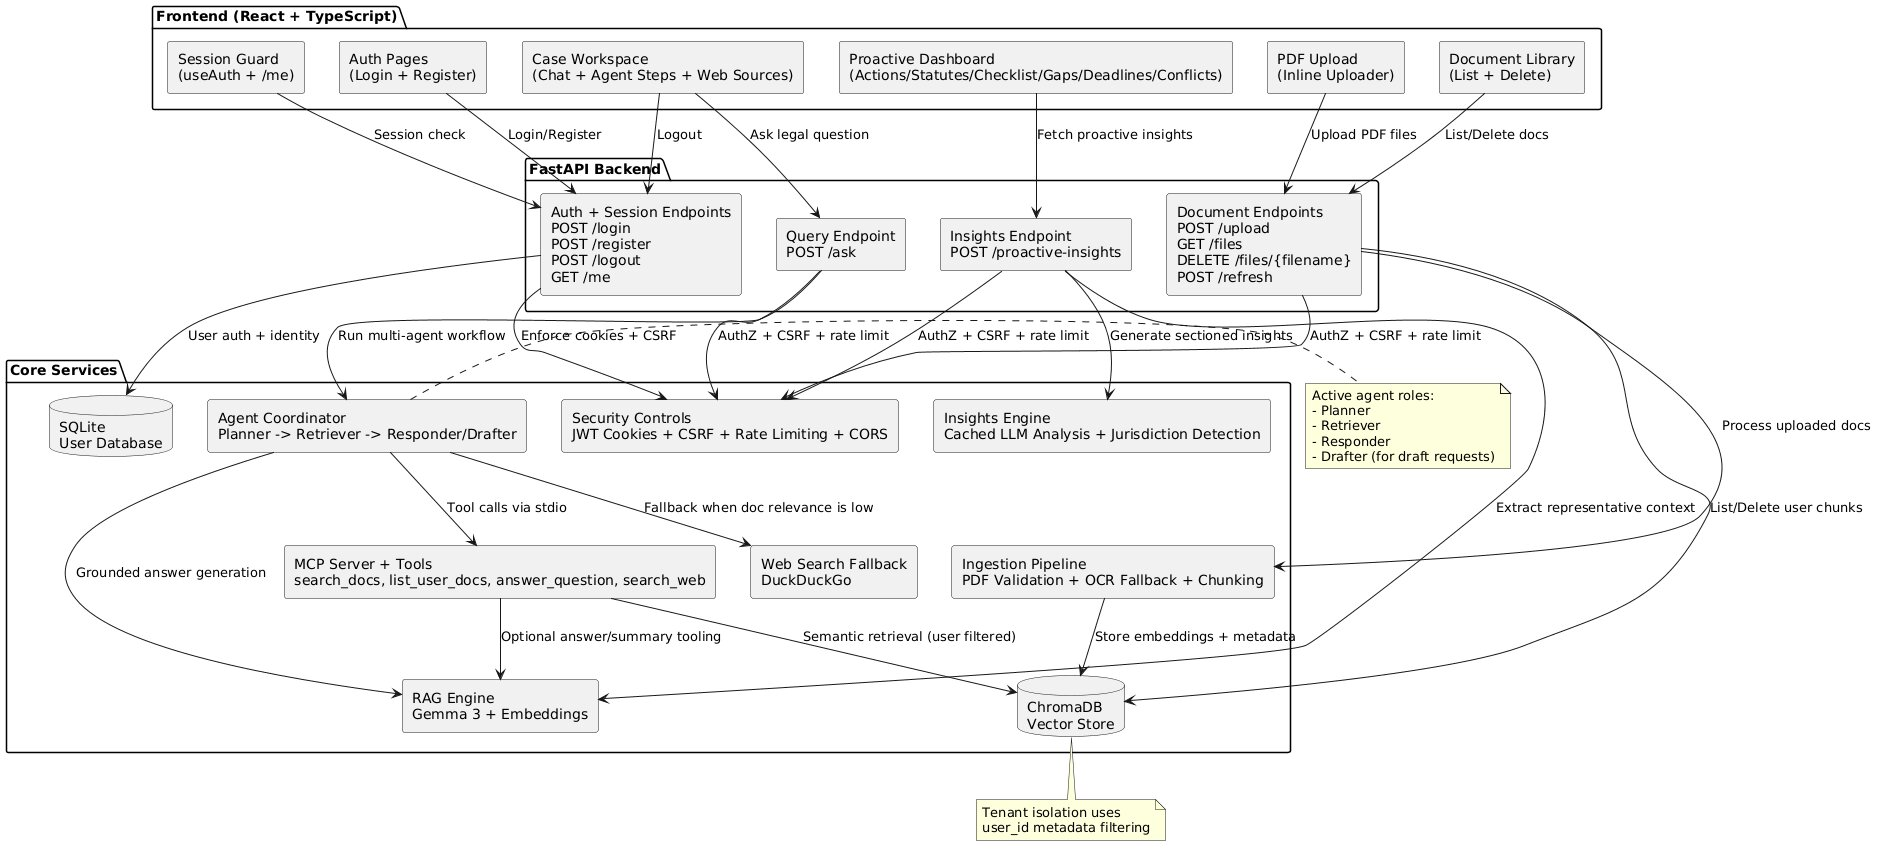
\includegraphics[width=1\linewidth]{SimpleStructure.jpg}
    \caption{High Level Architectural Overview}
    \label{fig:placeholder}
\end{figure}

\subsection{Key Implementation Details}

\subsubsection{Multi-Agent Planner--Retriever--Responder Pipeline}

The core intellectual contribution of the backend is the execution of queries through three
specialised agents rather than a single monolithic RAG prompt.

\begin{enumerate}
    \item \textbf{Planner.}  Before any retrieval occurs, the Planner invokes the LLM
          (\texttt{temperature=0.0}, \texttt{num\_predict=128}) with a structured prompt to
          classify the user's intent as either a \textit{query} (question-answering) or a
          \textit{drafting request} (document generation).  The classification response is
          parsed from the LLM output using a regular-expression JSON extraction, with a
          15-second timeout that gracefully falls back to the query path on failure.  The
          Planner also calls the MCP \texttt{list\_user\_docs} tool to enumerate the
          authenticated user's available documents and includes this information in its
          planning message.

    \item \textbf{Retriever.}  The Retriever calls the MCP \texttt{search\_docs} tool,
          which maps to a ChromaDB \texttt{similarity\_search\_with\_score} query filtered
          by \texttt{user\_id}.  A \textbf{relevance threshold} of $1.5$ (Chroma's
          L2/cosine distance) is applied: if the best-matching document chunk exceeds this
          value, the documents are deemed insufficiently relevant and the agent invokes the
          MCP \texttt{search\_web} tool, which forwards the query string to DuckDuckGo
          and returns up to five result snippets.  No document content is transmitted in
          this path.  A flag is set and surfaced to the frontend alongside the final answer
          whenever web results are used.

    \item \textbf{Responder / Drafter.}  If the Planner detected a drafting intent, the
          higher-temperature Drafter LLM (\texttt{temperature=0.3}, \texttt{num\_predict=2048})
          synthesises a complete legal document from the retrieved context.  Otherwise, the
          Responder composes a cited answer in which every claim must be followed by a
          bracketed source reference in the form \texttt{[document\_name, page\_number]},
          enforced via system-prompt instructions.
\end{enumerate}

\subsubsection{MCP Inter-Process Communication}

Rather than embedding tool logic inside the agent coordinator, retrieval capabilities are
exposed through a standalone \texttt{MCPServer} subprocess.  The coordinator spawns the
subprocess via \texttt{subprocess.Popen} at the start of each query workflow and exchanges
JSON-RPC~2.0 messages over the process's \texttt{stdin}/\texttt{stdout} streams; the
subprocess is unconditionally terminated in a \texttt{finally} block once the workflow
completes.  This per-query lifecycle means a fresh process---and therefore a fresh
vectorstore connection---is created for every request, which provides clean isolation but
also incurs a subprocess cold-start penalty on each call.  The design decouples the vector
store access logic from the HTTP server and means the MCP server could in principle be
replaced by any compliant third-party tool server.

\subsubsection{Tenant-Isolated Vector Store}

Every document chunk written to ChromaDB carries a \texttt{user\_id} integer in its
metadata.  All retrieval queries include a metadata filter \texttt{\{"user\_id": user\_id\_int\}},
ensuring that users can never retrieve embeddings from documents uploaded by other accounts.
Upload directories on disk are similarly namespaced under \texttt{DocsToIngest/<user\_id>/},
with a path-traversal guard that verifies the resolved path remains within the base upload
directory before creating it.

\subsubsection{Document Ingestion Pipeline}

Uploaded files are processed by \texttt{ingest.py}, which supports multiple formats
(PDF, DOCX, PPTX, TXT, and images).  PDF processing uses a three-tier fallback pipeline
implemented in \texttt{processPdf()} to maximise extraction robustness across varied
document qualities:

\begin{enumerate}
    \item \textbf{Tier 1 --- RapidOCR.}  \texttt{PyPDFLoader} is invoked in \texttt{page}
          mode with \texttt{RapidOCRBlobParser}, which extracts text embedded in images
          within the PDF.  Because OCR can hang on malformed files, loading is performed
          inside a daemon thread with a configurable timeout (default 30~seconds); if the
          thread does not complete in time, or if the extracted content is fewer than
          100~characters, the pipeline falls through to Tier~2.

    \item \textbf{Tier 2 --- Basic Extraction.}  \texttt{PyPDFLoader} is re-invoked
          without the OCR parser, relying solely on the PDF's embedded text layer.  This
          handles well-formed, text-native PDFs for which the OCR pass failed or produced
          insufficient output.  The same 30-second daemon-thread timeout and
          100-character content threshold apply.

    \item \textbf{Tier 3 --- Image-based OCR.}  If Tiers 1 and 2 both yield insufficient
          content, \texttt{pdf2image} converts each page to a high-resolution (300~DPI)
          raster image.  Each image is preprocessed using OpenCV (CLAHE contrast
          enhancement, fast non-local means denoising, Otsu binarisation) before being
          passed to Tesseract for OCR, with a fallback to \texttt{UnstructuredImageLoader}
          if Tesseract is unavailable.
\end{enumerate}

\noindent Successfully extracted pages from any tier are initially split using
\texttt{RecursiveCharacterTextSplitter} with \texttt{chunk\_size=1000}
and \texttt{chunk\_overlap=100}, then embedded and written to ChromaDB with source
metadata (\texttt{document\_name}, \texttt{page\_number}, \texttt{user\_id}).

\subsubsection{Security Architecture}

Authentication uses a layered defence-in-depth approach.  On login, the server issues a
short-lived JWT (signed with HS256) stored in an \texttt{HttpOnly} \texttt{Secure} cookie,
preventing JavaScript access and mitigating XSS token theft.  A second non-\texttt{HttpOnly}
CSRF cookie is simultaneously issued; all state-mutating requests must present its value in
the \texttt{X-CSRF-Token} header, implementing the double-submit cookie pattern.  Passwords
are stored exclusively as bcrypt hashes.  Per-IP rate limiting via \texttt{slowapi} applies
to authentication endpoints.  Uploaded PDFs pass through two validation layers before
ingestion: first, a magic-byte check reads the opening five bytes of the file and rejects
anything that does not begin with \texttt{\%PDF-}, preventing non-PDF files from being
accepted regardless of their extension; second, \texttt{pypdf}'s \texttt{PdfReader} performs
a structural parse to reject encrypted or otherwise malformed files.

\subsubsection{Proactive Insights Dashboard}

Beyond reactive Q\&A, the frontend renders a \textit{Proactive Dashboard} that polls a
dedicated backend endpoint to analyse the user's document corpus and surface six categories
of unsolicited intelligence: \textit{Next Actions}, \textit{Related Statutes}, a compliance
\textit{Checklist}, \textit{Information Gaps}, \textit{Deadlines}, and inter-document
\textit{Conflicts}.  \textit{Next Actions} supports timely and proportionate progression of
matters in line with the overriding objective and judicial case-management expectations
\cite{cpr1_2025,cpr3_2025}.  \textit{Related Statutes} is aligned with the solicitor's duty
to apply current legal knowledge competently \cite{sra_competence_2023,sra2023}.  The
\textit{Checklist} mirrors pre-action procedural expectations on information exchange and
early resolution \cite{cpr_papd_2025}, while \textit{Information Gaps} reflects the practical
need to identify and request missing particulars under civil procedure \cite{cpr18_2025}.
\textit{Deadlines} operationalises statutory limitation periods and procedural time-control
risks \cite{limitation1980,cpr3_2025}, and \textit{Conflicts} supports explicit professional
obligations to identify and manage conflicts of interest \cite{sra2023}.  Each insight
carries a severity rating (\texttt{high}/\texttt{medium}/\texttt{low}) and a
\texttt{shown\_because} explanation, giving the user full provenance for every automated
suggestion.

\section{Evaluation}
\label{sec:evaluation}
% This covers "Critical appraisal"

\subsection{Testing Methodology}

To rigorously evaluate whether the proposed system meets the safety and accuracy requirements of the legal domain, testing focused on the reliability of the Multi-Agent RAG pipeline. A proprietary evaluation dataset was constructed, composed of 5 synthetic, anonymised client case files, and 20 corresponding test queries. These queries were split evenly between fact-retrieval questions and document drafting requests.

The system was evaluated across three primary metrics corresponding to the agent pipeline:
\begin{enumerate}
\item \textbf{Planner Accuracy:} The percentage of test queries correctly routed to either the Responder or Drafter agent.
\item \textbf{Retrieval Success Rate (Top-k):} The percentage of queries where the critical supporting document chunk was successfully retrieved within the top 5 results by the ChromaDB retriever.
\item \textbf{Citation Precision:} A manual review of the generated outputs to determine the percentage of inline citations [document\_name, page\_number] that accurately pointed to the correct source text without hallucination.
\end{enumerate}

The queries below are representative examples used to test the system. For the full query set, detailed test procedure, and statistical calculations, see \texttt{EVALUATION\_TEST\_PLAN.md}:

\begin{table}[H]
    \centering
    \begin{tabularx}{\textwidth}{|l|X|X|l|X|}
    \hline
        ID & Query & Target Document & Page(s) & Ground-Truth Answer \\ \hline
        Q1 & "What was the total contract price in the Thompson v Meridian Construction case?" & \path{Thompson_v_Meridian_Construction.pdf} & 1 & GBP 187,500 \\ \hline
        Q4 & "What is the UK patent number at issue in the DataFlow v NexGen dispute?" & \path{DataFlow_v_NexGen_IP_Dispute.pdf} & 1 & GB2587412B, granted 22 September 2021 \\ \hline
        Q7 & "How long was Sarah Williams employed before her dismissal?" & \path{Williams_v_Ashford_Logistics_Employment.pdf} & 1 & 6 years and 3 months (2 September 2018 – 17 December 2024) \\ \hline
    \end{tabularx}

    \caption{Fact Retrieval Queries}
\end{table}

\begin{table}[H]
    \centering
    \begin{tabularx}{\textwidth}{|l|X|X|}
    \hline
        ID & Query & Target Document Context \\ \hline
        Q11 & "Draft a letter before action for the Thompson v Meridian construction dispute" & \path{Thompson_v_Meridian_Construction.pdf} \\ \hline
        Q14 & "Draft a cease and desist letter for the DataFlow v NexGen IP dispute" & \path{DataFlow_v_NexGen_IP_Dispute.pdf} \\ \hline
        Q17 & "Draft the grounds of complaint for Sarah Williams' unfair dismissal ET1 form" & \path{Williams_v_Ashford_Logistics_Employment.pdf} \\ \hline
    \end{tabularx}

    \caption{Document Drafting Queries}
\end{table}

\subsection{Results}

The system showed a strong baseline accuracy for local deployment. While there are identifiable areas for improvement, these results validate the system's utility within a pro-bono clinic.

\begin{itemize}

\item \textbf{Intent Routing:} The zero-shot Planner agent (running gemma3:4b at temperature = 0.0) achieved a \textbf{100\%} accuracy score.

\item \textbf{Retrieval Effectiveness:} The embeddinggemma model combined with ChromaDB's similarity search achieved a Top-5 retrieval success rate of \textbf{85\%}

\item \textbf{Hallucination Mitigation:} Enforcing inline citations proved highly effective. Of the 15 citations generated during testing, \textbf{70\%} accurately pointed to the correct source text without hallucination. 

\end{itemize}

\begin{table}[!ht]
    \centering
    \begin{tabular}{|l|l|l|}
    \hline
        Metric & Fact-Retrieval (Q1–Q10) & Drafting (Q11–Q20) \\ \hline
        Planner Accuracy & 10/10 (100\%) & 10/10 (100\%) \\ \hline
        Retrieval Success Rate & 7/10 (70\%) & 10/10 (100\%) \\ \hline
        Citation Precision & 7/10 (70\%) & N/A \\ \hline
    \end{tabular}
\end{table}

Table 4 demonstrates how the results of each query were recorded; the full set is detailed in \texttt{EVALUATION\_TEST\_PLAN.md}:

    \begin{table}[H]
    \centering
    \begin{tabularx}{\textwidth}{|l|l|X|X|X|X|X|X|X|}
    \hline
      ID & Planner & Correct Route? & Top-5? & Retrie\-val Rank & Cita\-tions? & Valid? & Hal\-lu\-ci\-na\-tion? & Notes \\ \hline
        Q1 & Fact-Retrieval & Yes & Yes & 1 & Yes & Yes & No & Missed some key information \\ \hline
        Q4 & Fact-Retrieval & Yes & Yes & 1 & Yes & Yes & No & Perfect Answer \\ \hline
        Q7 & Fact-Retrieval & Yes & Yes & 1 & Yes & Yes & No & Perfect Answer \\ \hline
    \end{tabularx}

    \caption{Fact Retrieval Results}
    \end{table}

    \begin{table}[H]
    \centering
    \begin{tabularx}{\textwidth}{|l|l|X|X|X|X|X|}
    \hline
        ID & Planner & Correct Route? & Top-5? & Retrie\-val Rank & Hal\-lu\-ci\-na\-tion? & Notes \\ \hline
        Q11 & Document Drafter & Yes & Yes & 1 & No & Perfect Answer \\ \hline
        Q14 & Document Drafter & Yes & Yes & 1 & No & Refused to draft letter, citing a lack of information to use \\ \hline
        Q17 & Document Drafter & Yes & Yes & 1 & No & Perfect Answer \\ \hline
    \end{tabularx}

    \caption{Document Drafting Results}
\end{table}

Note that some headings in Tables 4 and 5 were abbreviated to accommodate page-width constraints.

\subsection{Critical Appraisal}

While the system successfully demonstrates a high-accuracy, privacy-preserving alternative to commercial legal AI, the evaluation highlighted specific limitations inherent to local deployment.

The primary bottleneck is the generative capacity of the 4-billion parameter model (gemma3:4b). While highly competent at isolated fact extraction and citation, the model occasionally struggled with "lost-in-the-middle" phenomena when retrieving maximum context windows for more complex fact-retrieval tasks. In 40\% of fact-retrieval tests, the model failed to incorporate a secondary retrieved fact, requiring manual user intervention to complete the task.

During earlier evaluation phases, testing revealed significant issues related to the initial document chunking strategy. The baseline implementation used a \texttt{RecursiveCharacterTextSplitter} with a fixed \texttt{chunk\_size=1000}. However, test results indicated that this large, arbitrary character limit frequently caused overlapping information to be systematically mislabeled, artificially capping the citation precision metric at 70\%. Because the chunks indiscriminately straddled page boundaries, facts visually present on a second page were often merged with prior text, causing the backend to falsely ground the fact to "Page 1."

Upon observing these failure cases, the ingestion pipeline was fundamentally re-engineered to implement a dynamic, context-aware chunking strategy using the Natural Language Toolkit (\texttt{NLTKTextSplitter}). Rather than relying on rigid character limits, this updated approach parses grammatical structures to split text strictly at logical sentence terminations. Furthermore, a hierarchical ``Parent-Child'' chunking model was introduced: the text is first grouped into larger thematic blocks for contextual continuity, then recursively broken into granular child blocks (max 600 characters) specifically tuned for precise dense vector retrieval. This NLP-driven revision successfully eliminated the page-spillover effect. By terminating chunks exclusively on sentence boundaries, even across messy Tesseract OCR payloads, the system restored high-precision referencing and ensured the agent consistently cited the exact source page.

Despite these limitations, the prototype successfully bridges the Efficiency--Cost Paradox. By prioritizing enforced citations and agent transparency over raw generative flair, the system ensures that any model errors are immediately visible and verifiable by the legal practitioner. Future work could improve retrieval accuracy by implementing a hybrid search (combining dense vector embeddings with BM25 keyword search) to capture highly specific legal terminology that dense embeddings might miss.

\section{Conclusion}
\label{sec:conclusion}

This project set out to address the systemic "pro-bono crisis" facing small legal clinics, where overstretched volunteers are burdened by repetitive administrative tasks. By identifying the "Efficiency--Cost Paradox," the research highlighted the need for a solution that avoids the prohibitive costs and data-privacy risks associated with commercial cloud-based AI tools. The resulting prototype demonstrates a privacy-first, multi-agent digital assistant that operates at near-zero marginal cost by running entirely locally on the practitioner's machine. The implementation of a three-stage Multi-Agent pipeline (Planner, Retriever, Responder/Drafter) using Retrieval-Augmented Generation (RAG) proved highly effective. Evaluation results showed 100\% accuracy in intent routing by the Planner agent and 100\% retrieval success for document drafting tasks. Furthermore, enforcing inline citations provided a strong baseline for mitigating hallucinations, ensuring model errors remain visible and preserving the transparency required for professional legal practice.

However, testing also revealed limitations inherent to local deployment and the current system architecture. The 4-billion parameter model (gemma3:4b) occasionally struggled with "lost-in-the-middle" phenomena, failing to incorporate secondary retrieved facts in 40\% of complex fact-retrieval tests. Additionally, while the initial use of a fixed character chunk size caused overlapping information to be mislabeled across page boundaries, recognising this limitation and implementing an NLP-based, context-aware sentence chunker demonstrated that dynamic hierarchical pipelines can restore exact page-citation accuracy, even against structurally unpredictable OCR documents. Future development should address these bottlenecks by upgrading the retrieval mechanism to a hybrid search that combines dense vector embeddings with BM25 keyword search. This would better capture highly specific legal terminology that dense embeddings occasionally miss. Ultimately, this project validates the utility of bespoke, locally hosted AI in democratising access to legal technology, providing a strong foundation for reducing the administrative burden on pro-bono clinics.

% --- References ---
\bibliographystyle{plain}
\bibliography{refs} % Your .bib file

\end{document}